\documentclass[12pt]{article}
\usepackage{amsmath}
\usepackage{tikz-dependency}
\DeclareMathOperator*{\argmax}{arg\,max}
\DeclareMathOperator*{\argmin}{arg\,min}
\DeclareMathOperator{\E}{\mathop{\mathbb{E}}}

\usepackage{hyperref}

\usepackage{amssymb}% http://ctan.org/pkg/amssymb
\usepackage{pifont}% http://ctan.org/pkg/pifont
\newcommand{\cmark}{\ding{51}}%
\newcommand{\xmark}{\ding{55}}%

\usepackage[english]{babel}
\usepackage[utf8]{inputenc}
\usepackage{bm}
\usepackage{graphicx}
\usepackage{tikz}
\usepackage{xcolor}
\usepackage{url}
\usepackage{rotating}
\usepackage{multirow}
\usepackage{natbib}
\usepackage{arydshln}

\newcommand{\key}[1]{\textbf{#1}}





\usepackage{mathtools}
\DeclarePairedDelimiter{\ceiling}{\lceil}{\rceil}

\title{Supplemental Materials for ``Universals of word order result from optimization of grammars for efficient communication''}
\author{
        Michael Hahn \\
                Department of Linguistics\\
       Stanford University
            \and
       Daniel Jurafsky\\
       Department of Linguistics\\
       Stanford University \\
       \and
       Richard Futrell\\
       Department of Language Science\\
       University of California, Irvine
}
\date{\today}

\begin{document}
\maketitle

\section{Results on all UD Relations}
Table~\ref{tab:all-predictions} shows the predicted prevalence of correlations between the \emph{obj} dependency and all UD dependency types, along with the expected prevalence according to typological studies.

\begin{table*} % TODO figure out away to make this table more aesthetic
	\begin{center}
	
\tiny{
\begin{tabular}{|l|l|l|ll|l|l|}
	\hline
	Relation & Real & DepL & Pred & Pars & Efficiency & Expected Prevalence  \\ \hline
% From Dryer	
acl  &  80   &   \textbf{85}$^{***}$   &   43   &   \textbf{82}$^{***}$   &   \textbf{71}$^{***}$  & $>50\%$  \citep{dryer1992greenbergian} \\
aux  &  12   &   \textbf{26}$^{***}$   &   \textbf{19}$^{***}$   &   49   &   \textbf{35}$^{**}$  & $<50\%$ \citep{dryer1992greenbergian} \\
lifted\_case  &  86   &   \textbf{81}$^{***}$   &   \textbf{40}$^{**}$   &   \textbf{77}$^{***}$   &   \textbf{67}$^{***}$ & $> 50 \%$ \citep{dryer1992greenbergian}  \\
lifted\_cop  &  94   &   \textbf{80}$^{***}$   &   59   &   \textbf{72}$^{***}$   &   \textbf{63}$^{**}$  & $> 50 \%$ \citep{dryer1992greenbergian} \\
lifted\_mark  &  76   &   \textbf{85}$^{***}$   &   \textbf{57}$^{*}$   &   \textbf{76}$^{***}$   &   \textbf{72}$^{***}$  & $> 50 \%$ \citep{dryer1992greenbergian} \\
nmod  &  80   &   \textbf{82}$^{***}$   &   49   &   \textbf{71}$^{***}$   &   \textbf{68}$^{***}$  & $> 50 \%$ \citep{dryer1992greenbergian} \\ 
obl  &  88   &   \textbf{78}$^{***}$   &   \textbf{71}$^{***}$   &   46   &   \textbf{68}$^{***}$  &  $> 50 \%$ \citep{dryer1992greenbergian} \\
xcomp  &  88   &   \textbf{90}$^{***}$   &   \textbf{76}$^{***}$   &   \textbf{89}$^{***}$   &   \textbf{85}$^{***}$  &  $> 50 \%$ \citep{dryer1992greenbergian} \\
\hdashline
nsubj  &  33   &   \textbf{29}$^{***}$   &   53   &   \textbf{7}$^{***}$   &   \textbf{23}$^{***}$  & $> 50 \%$ \citep{dryer1992greenbergian} \\
advmod  &  35   &   51   &   \textbf{18}$^{***}$   &   47   &   \textbf{39}$^{**}$  & $>50\%$ for manner adverbs; $\approx 50\%$ for negation, TAM, intensifiers \citep{dryer1992greenbergian} \\

\hline
% Other universals, not in Dryer
advcl  &  86   &   \textbf{84}$^{***}$   &   51   &   \textbf{67}$^{***}$   &   \textbf{67}$^{*}$  & $>50\%$ \citep{greenberg1963universals,diessel2001ordering} \\
amod  &  51   &   \textbf{84}$^{***}$   &   42   &   \textbf{53}$^{*}$   &   51   & $\approx 50\%$ \citep{dryer1992greenbergian} \\
nummod  &  37   &   \textbf{74}$^{**}$   &   49   &   52   &   52 & $\approx 50\%$ \citep[][89A vs. 83A]{wals} \\

\hline
% Typological data not available
appos  &  77   &   \textbf{77}$^{***}$   &   49   &   \textbf{67}$^{***}$   &   \textbf{62}$^{**}$ &  Unknown \\%($>50\%$? correlates with \textit{nmod} according to Greenberg U 23)  \\ % \cite{cinque2009greenberg} claims it correlates with OV/VO. However, it's not clear to me how closely appos matches the subject of the typological claim
lifted\_cc  &  71   &   \textbf{83}$^{***}$   &   51   &   \textbf{81}$^{***}$   &   \textbf{71}$^{***}$  & Unknown \\
ccomp  &  86   &   \textbf{88}$^{***}$   &   \textbf{70}$^{**}$   &   \textbf{77}$^{***}$   &   \textbf{77}$^{**}$ & Unknown (cf. \cite{dryer1980positional}) \\ % TODO According to Dryer 1980, there is a correlation
csubj  &  79   &   \textbf{78}$^{***}$   &   60   &   \textbf{66}$^{***}$   &   \textbf{68}$^{**}$  & Unknown (cf. \cite{dryer1980positional}) \\% TODO According to Dryer 1980, there is a correlation
expl  &  12   &   36   &   62   &   40   &   53  & Unknown \\
iobj  &  74   &   49   &   \textbf{78}$^{***}$   &   \textbf{38}$^{*}$   &   62  & Unknown \\
vocative  &  46   &   \textbf{42}$^{*}$   &   59   &   45   &   \textbf{45}$^{*}$  & Unknown \\

\hline
% Uninterpretable
compound  &  66   &   \textbf{61}$^{*}$   &   48   &   \textbf{58}$^{*}$   &   52  & Uninterpretable \\
det  &  31   &   \textbf{71}$^{***}$   &   \textbf{56}$^{*}$   &   48   &   54  & Uninterpretable (conflates articles and others) \\%$.50\%$ for articles, $\approx 50\%$ for others, \citep{dryer1992greenbergian} \\ %TODO what else is conflated in det? why do we keep advmod but not det?
dislocated  &  47   &   61   &   \textbf{68}$^{**}$   &   55   &   58  & Uninterpretable \\
dep  &  56   &   \textbf{64}$^{*}$   &   52   &   58   &   \textbf{58}$^{*}$   & Uninterpretable \\

\hline
% UD artifacts
conj  &  72   &   \textbf{82}$^{***}$   &   \textbf{42}$^{**}$   &   \textbf{62}$^{***}$   &   \textbf{59}$^{*}$  & UD artifact  \\
discourse  &  24   &   \textbf{36}$^{**}$   &   \textbf{41}$^{*}$   &   49   &   46  & UD artifact   \\
fixed  &  78   &   \textbf{32}$^{***}$   &   45   &   47   &   44  & UD artifact   \\
flat  &  73   &   \textbf{66}$^{**}$   &   45   &   \textbf{59}$^{**}$   &   54  & UD artifact   \\
goeswith  &  61   &   57   &   44   &   57   &   52  & UD artifact   \\
list  &  94   &   59   &   50   &   54   &   52  & UD artifact  \\
orphan  &  82   &   \textbf{70}$^{**}$   &   50   &   \textbf{55}$^{*}$   &   59  & UD artifact   \\
parataxis  &  66   &   56   &   43   &   57   &   59  & UD artifact  \\
reparandum  &  18   &   53   &   57   &   43   &   48  & UD artifact  \\


 \hline
%comp. &
%\multirow{3}{*}{NP}&
%	AP &
    \multicolumn{7}{l}{\footnotesize{Significance levels: $^*$: $p < 0.05$, $^{**}$: $p < 0.01$, $^{***}$: $p < 0.001$}}
\end{tabular}
}

\end{center}
\caption{Predictions on all UD relations occurring in more than one language. Numbers are the fraction of languages where the direction of the given relation agrees in direction with the \emph{obj} relation. In the last column, we indicate what direction would be expected typologically. ``Uninterpretable'' UD relations are those which collapse so many different linguistic relationships that they are not linguistically meaningful. ``UD artifact'' relations are those whose order is determined strictly by UD parsing standards, such that their order is not linguistically meaningful: these include dependencies such as the connection between two parts of a word that have been separated by whitespace inserted as a typo (\emph{goeswith}).}
\label{tab:all-predictions}
\end{table*}

\section{Results on Best Optimized Grammars}

In the main part, we reported the percentage of optimized grammars supporting correlations.
Here we report these numbers for the grammars that optimize each objective most successfully.
That is, for each language and objective, we chose among the eight optimized grammars the one that achieves the best value for the objective function on the validation partition of the treebanks -- that is, the one where the optimization procedure was most successful.

Numbers for these languages are shown in Table~\ref{table:results-dryer-best-only}.
%Confirming the results from the main paper, 
As expected, the correlations mostly have stronger prevalences than when considering all optimized languages.
For Dependency Length, the correlations that it predicts mostly have prevalences close to 100 \%, whereas both the UD languages and efficiency-optimized languages show somewhat lower percentages.
That is, dependency length mostly overshoots for the correlations that it predicts correctly.

\begin{table*}
	\begin{center}
\begin{tabular}{|ll|l|l|l|ll|l|}
	\hline
	%&
	\multicolumn{2}{|c|}{Correlates with...}   &          \multirow{2}{*}{Operationalization}       &     \multirow{2}{*}{Real}   & \multirow{2}{*}{DepL}  & \multirow{2}{*}{Pred}   &  \multirow{2}{*}{Pars} &  \multirow{2}{*}{Efficiency}  \\ 
	verb & object &      & & & &  & \\ \hline \hline % \textsc{verb} $\xrightarrow{obj}$ \textsc{noun}
%adp. &
adposition    &    NP    &    lifted\_case    &    86    &    98    &    69    &    88    &    83   \\
copula    &    NP    &    lifted\_cop    &    94    &    98    &    58    &    85    &    74   \\
auxiliary    &    VP    &    aux    &    88    &    84    &    90    &    61    &    73   \\
noun    &    genitive    &    nmod    &    80    &    98    &    75    &    88    &    91   \\
noun    &    relative clause    &    acl    &    80    &    100    &    69    &    88    &    90   \\
complementizer    &    S    &    lifted\_mark    &    76    &    100    &    76    &    82    &    87   \\
verb    &    PP    &    obl    &    88    &    98    &    88    &    75    &    91   \\
want    &    VP    &    xcomp    &    88    &    100    &    92    &    94    &    96   \\
verb    &    subject    &    nsubj    &    33    &    25    &    53    &    10    &    21   \\
verb    &    manner adverb    &    advmod    &    35    &    61    &    27    &    55    &    36   \\
 \hline
%comp. &
%\multirow{3}{*}{NP}&
%	AP &
\end{tabular}
	\end{center}
	\caption{Percentages of grammars supporting correlations, among grammars that best optimize each objective on treebanks of a given language.}\label{table:results-dryer-best-only}
\end{table*}


\begin{figure}
    \centering
    
    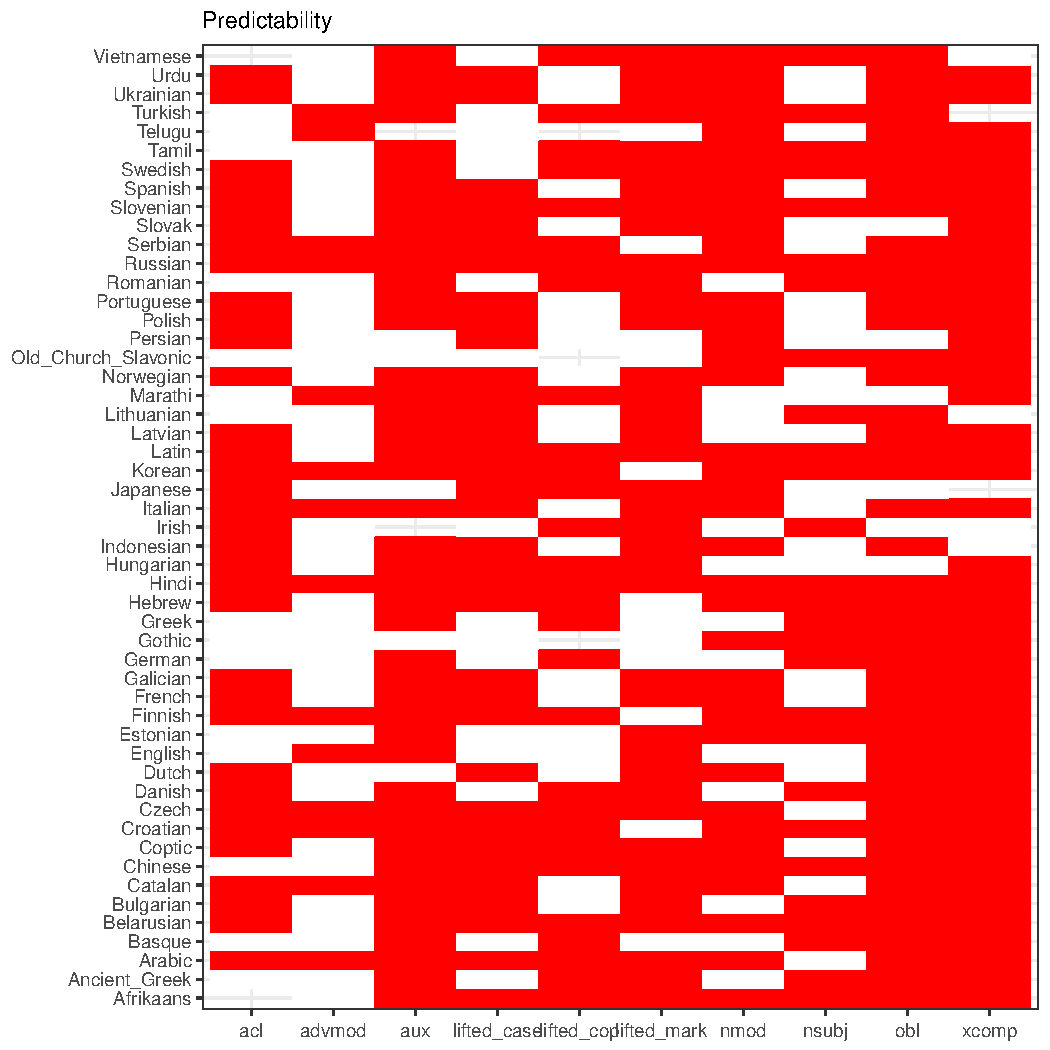
\includegraphics[scale=.25]{figures/coverage-langmod-best.pdf}
    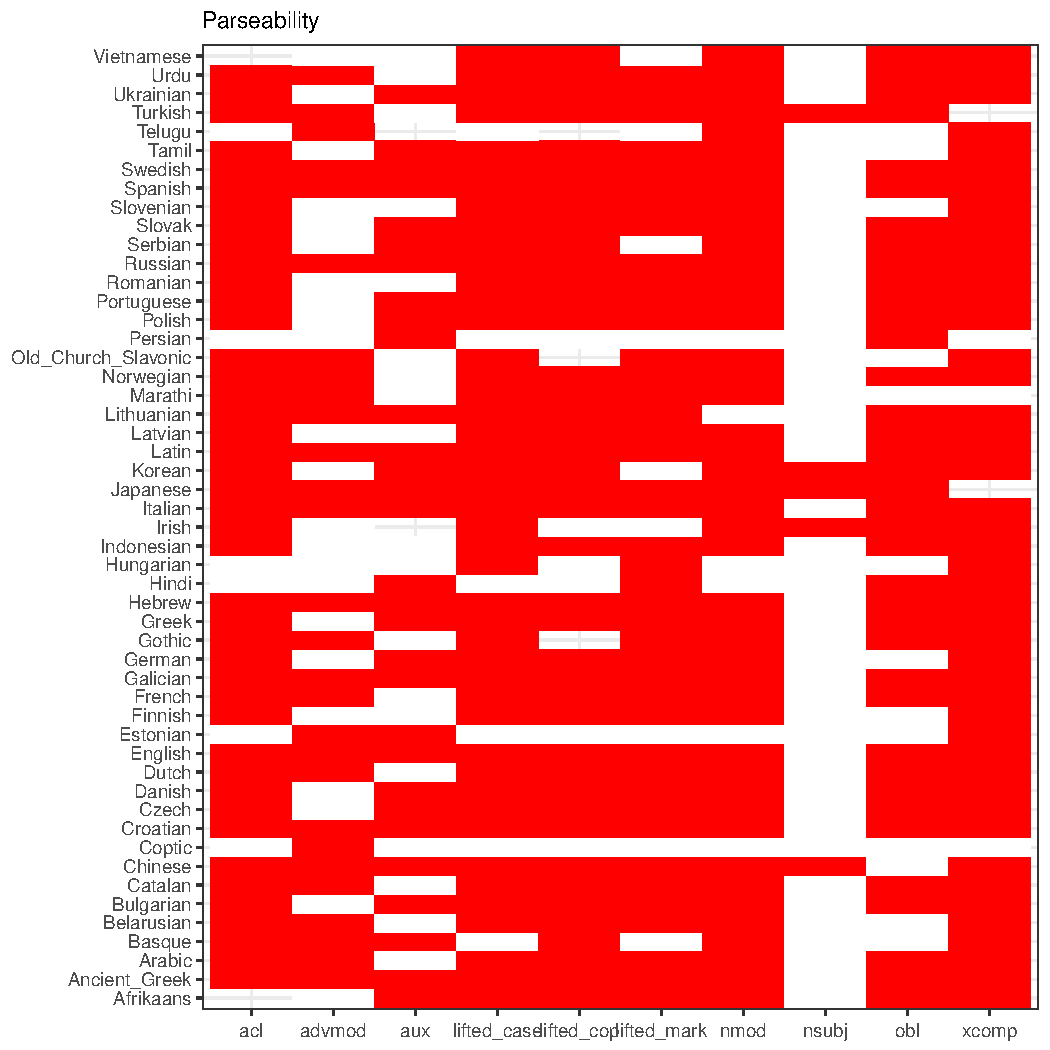
\includegraphics[scale=.25]{figures/coverage-parse-best.pdf}
    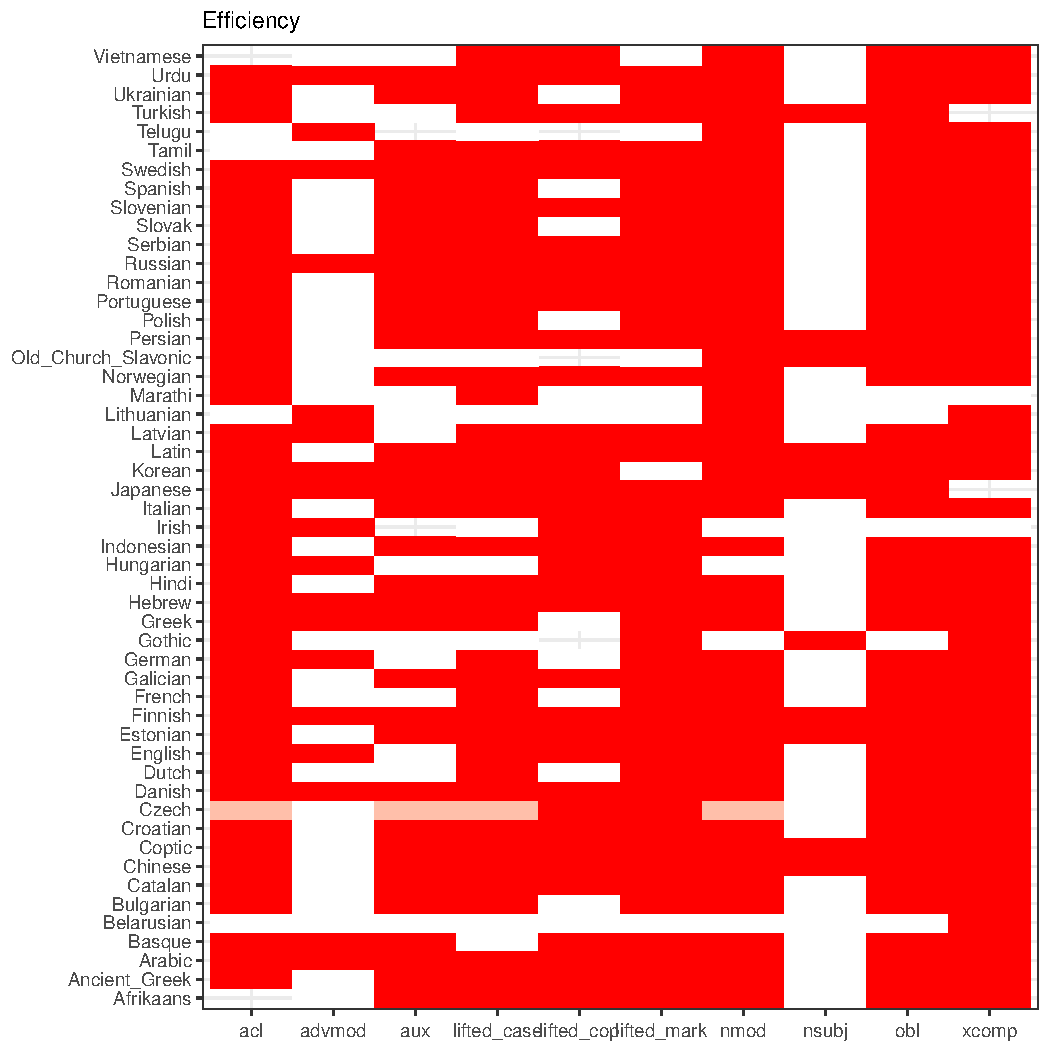
\includegraphics[scale=.25]{figures/coverage-two-lambda09-best.pdf}
    
    
    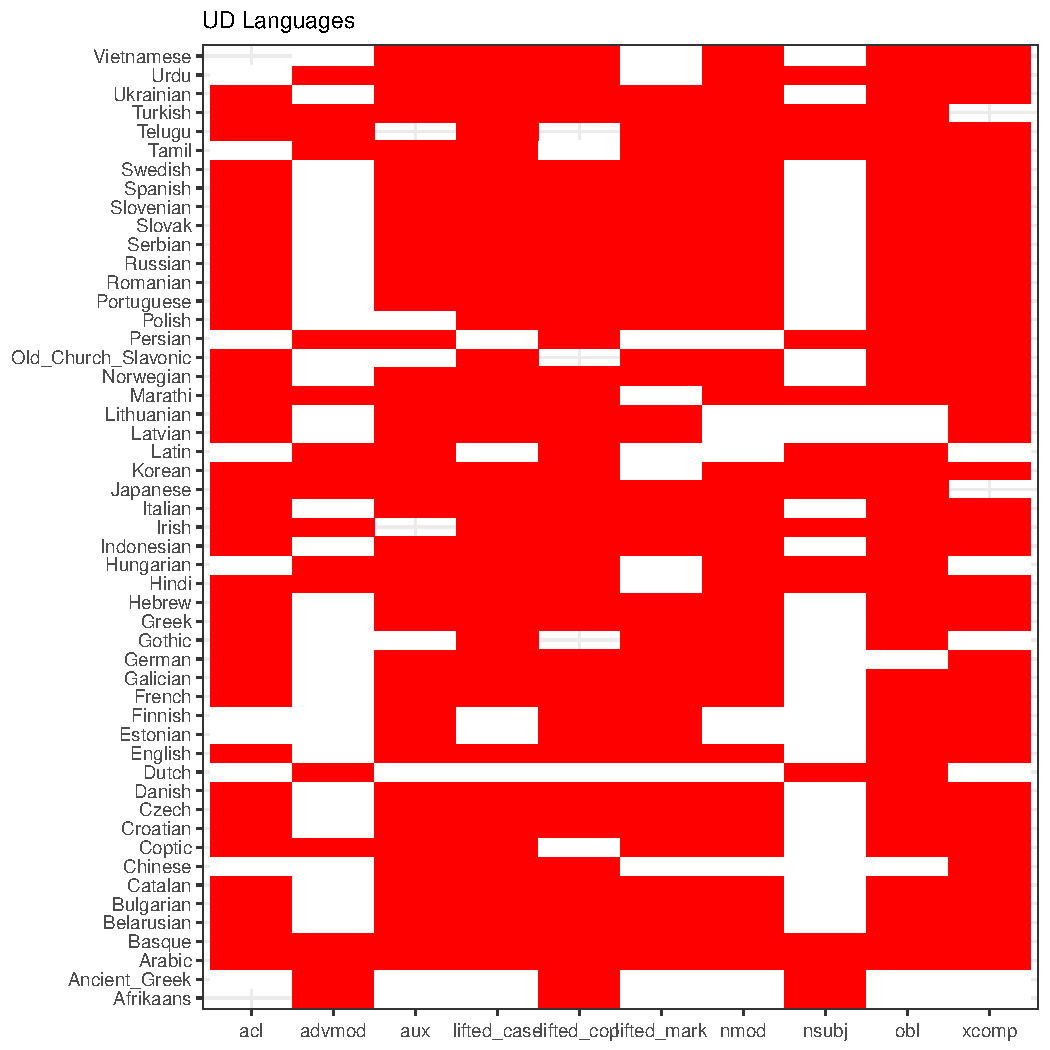
\includegraphics[scale=.25]{figures/coverage-ground.pdf}
    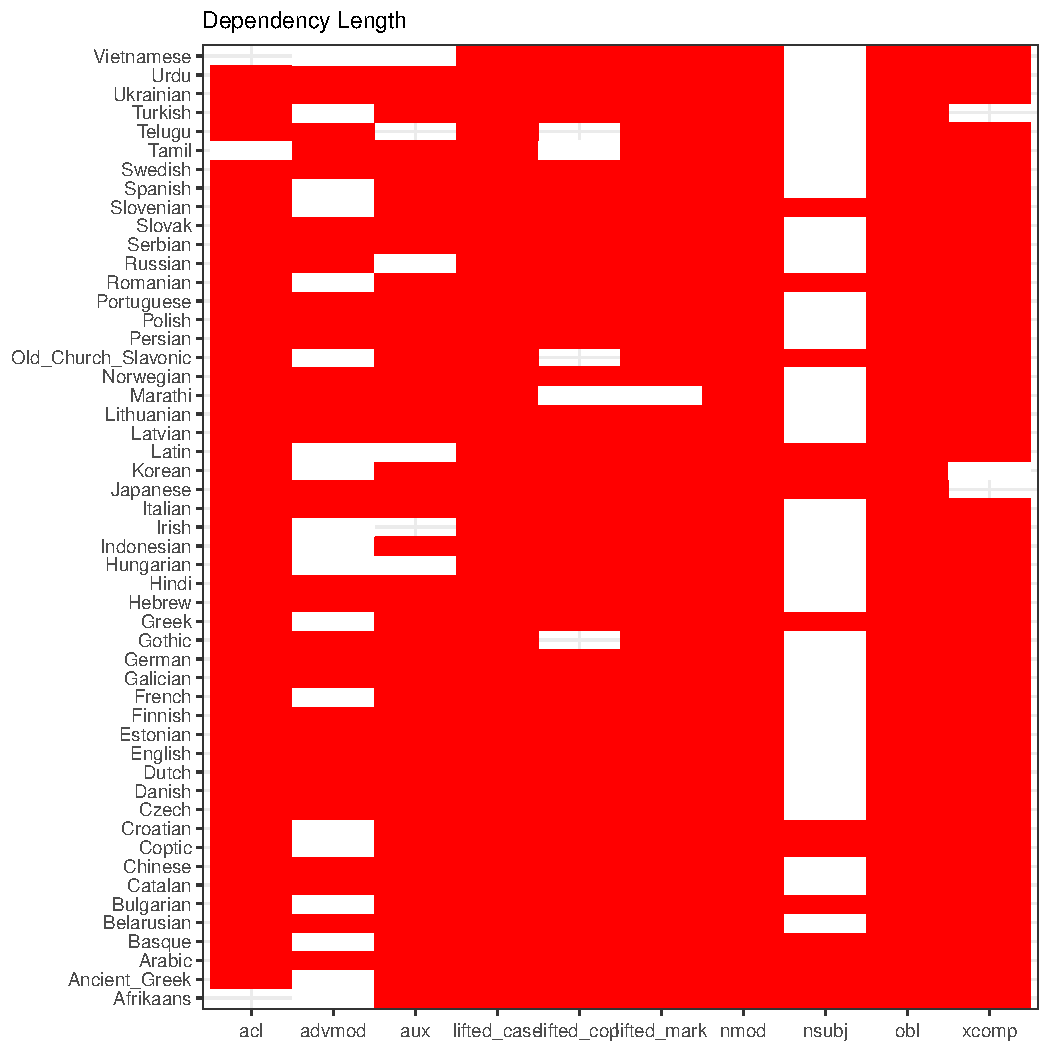
\includegraphics[scale=.25]{figures/coverage-depl.pdf}
	\caption{Correlations satisfied by the best word order grammars for predictability, parseability, efficiency, by the UD languages, and by the best grammars for dependency length.}
    \label{fig:posterior-prevalence}
\end{figure}


\section{Further Statistical Analyses}

In the main results table, we reported the fraction of optimized languages satisfying a correlation.
We show that essentially the same predicted fractions are obtained when controlling for the imbalance in distribution of language families.

To this end, we used the logistic mixed-effects regressions that were used to estimate significance to compute the expected prevalence of a correlation controlling for language families.
To obtain predictions controlling for languages and language families, we plot the logit-transformed posterior of $\alpha$ in Figure \ref{fig:posterior-prevalence}.



\begin{figure}
    \centering
    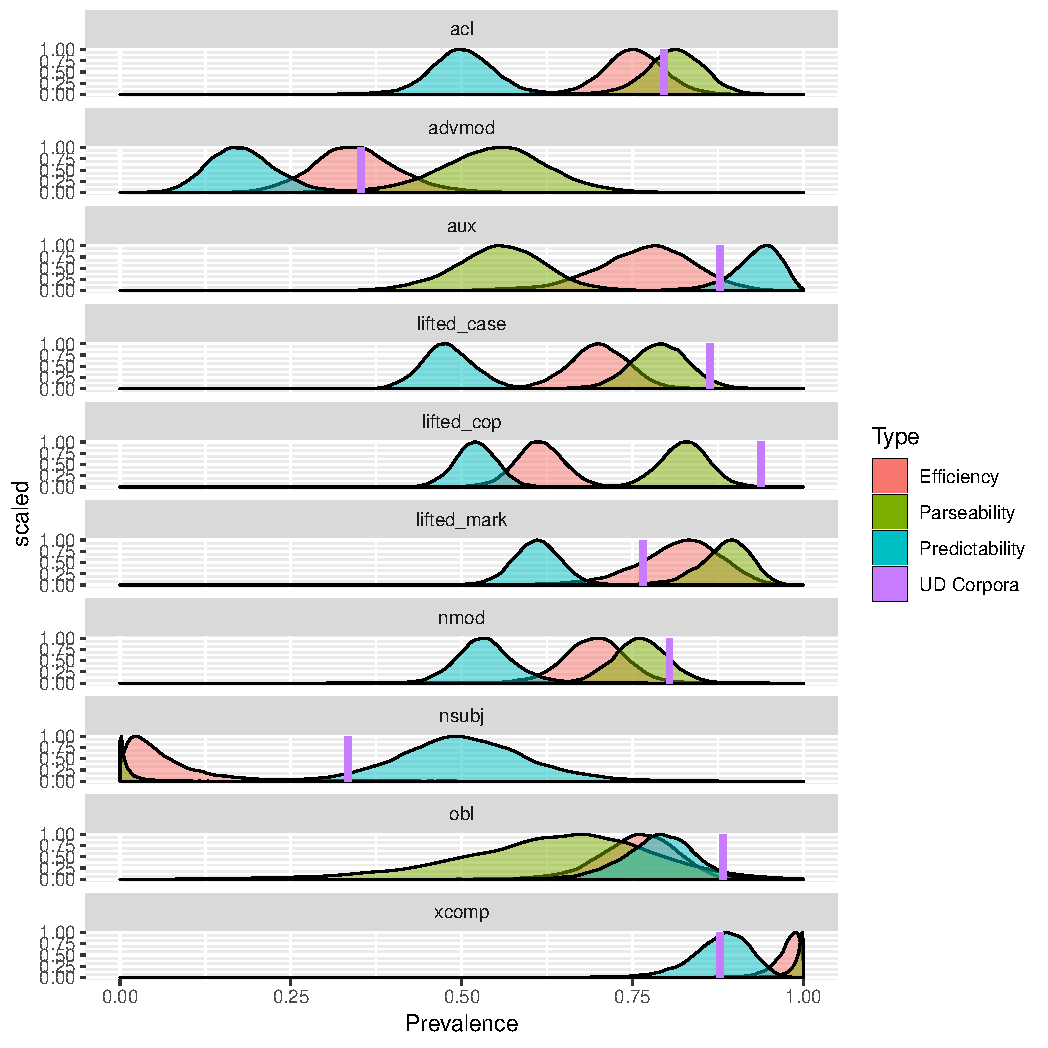
\includegraphics[scale=.7]{figures/posterior_joint_with_ud.pdf}
	\caption{Posteriors of the prevalences of the correlations among languages optimized for Predictability (red), parseability (green), and efficiency (blue), controlling for languages and language families, with prevalence in the UD languages.}
    \label{fig:posterior-prevalence}
\end{figure}



%\begin{figure}
%    \centering
%    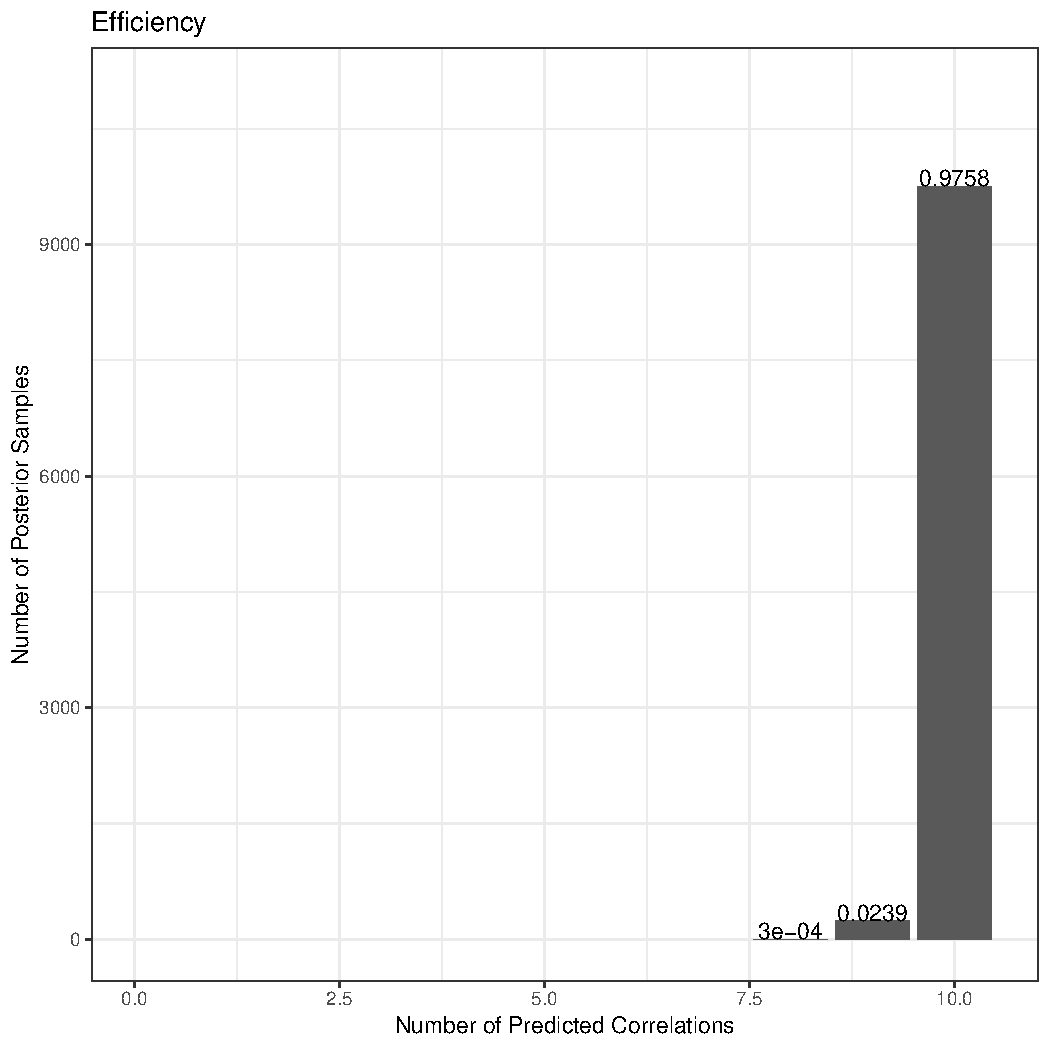
\includegraphics[scale=.3]{figures/posterior-satisfied-universals-efficiency.pdf}
%     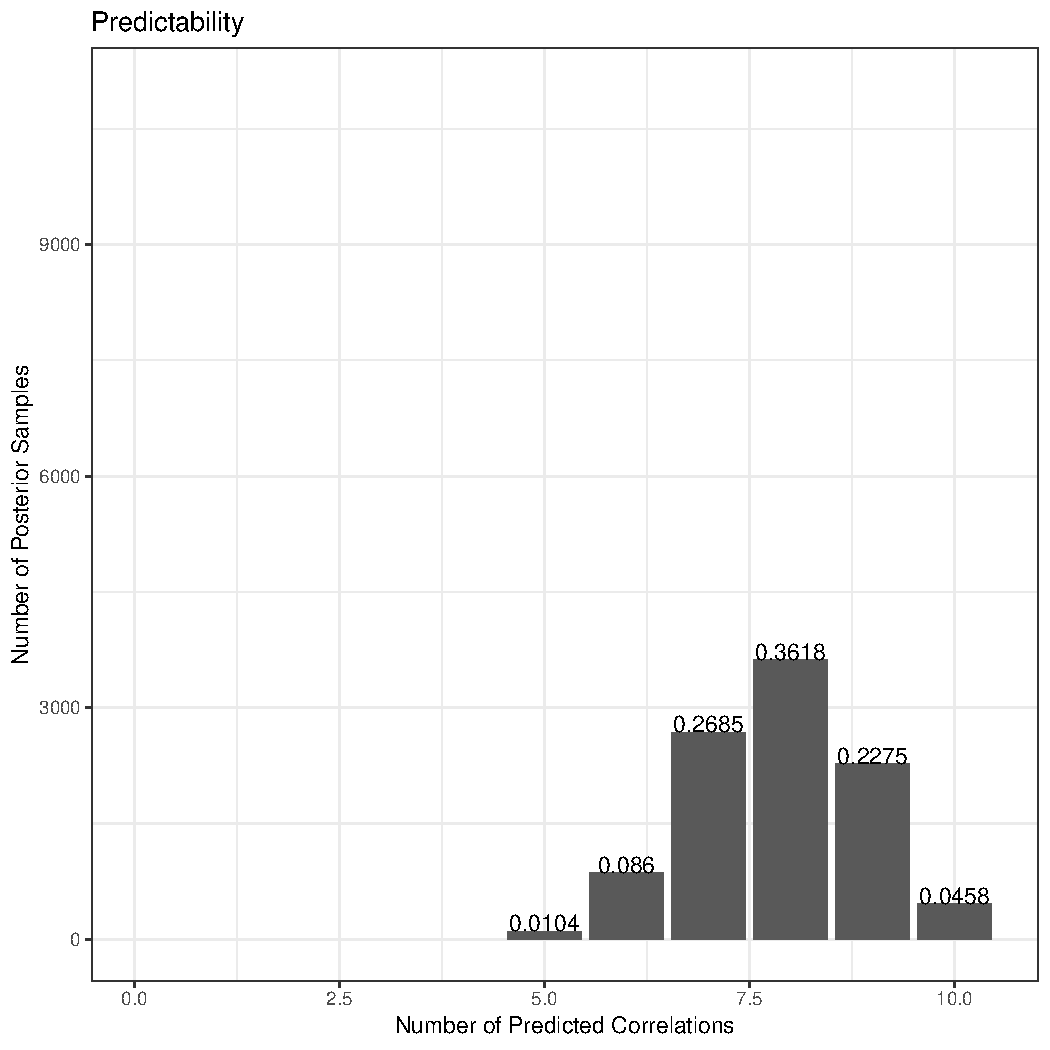
\includegraphics[scale=.3]{figures/posterior-satisfied-universals-langmod.pdf}
%     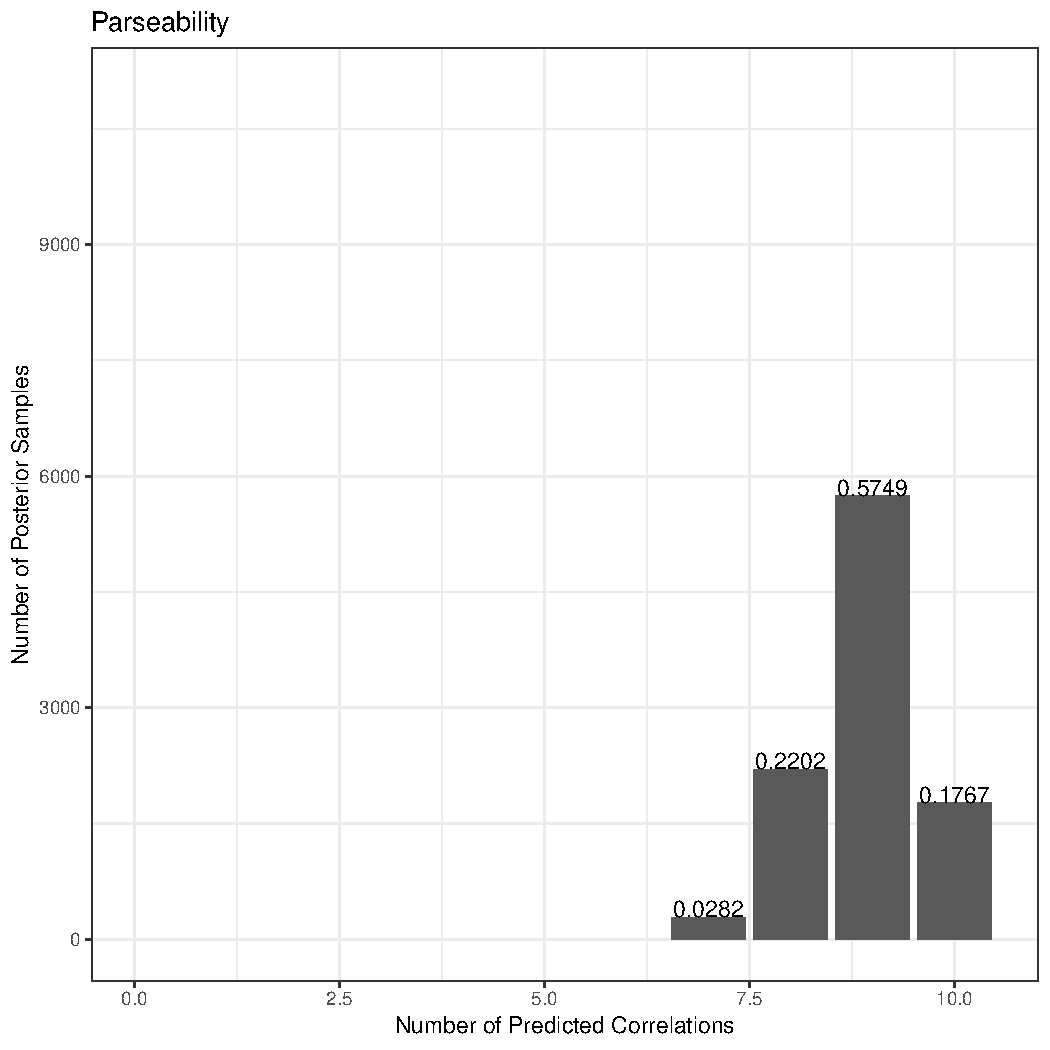
\includegraphics[scale=.3]{figures/posterior-satisfied-universals-parseability.pdf}
%    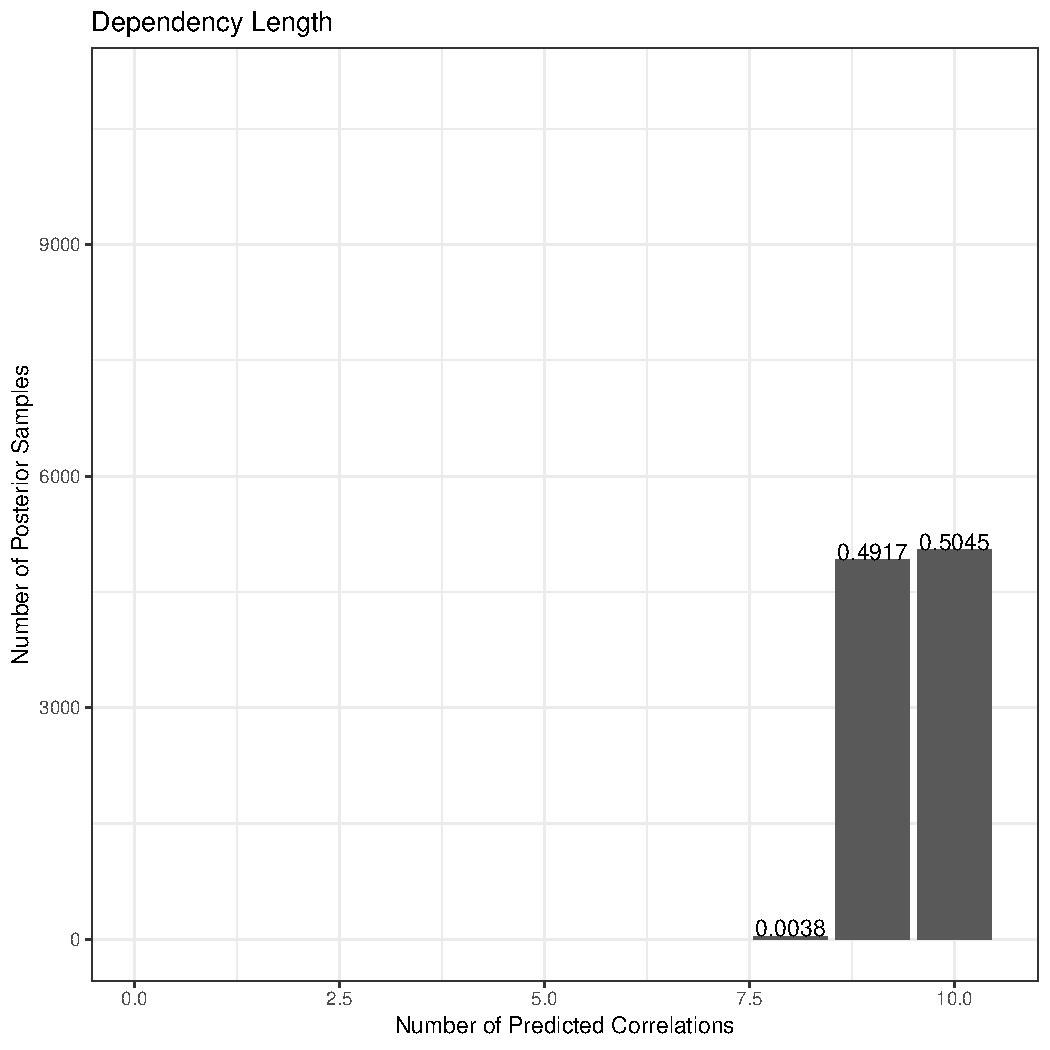
\includegraphics[scale=.3]{figures/posterior-satisfied-universals-depl.pdf}
%	\caption{Posterior of the number of correlations predicted in the direction found in the UD treebanks.}
%    \label{fig:posterior-satisfied-count}
%\end{figure}



%We argued that efficiency predicts all 10 correlation universals in the direction manifested in the UD corpora, as for each universal, the posterior probability that less than $50 \%$ of the optimized grammars satisfy the correlation was less than $0.05$.
%To address potential multiple comparisons problems, we use a single logistic model to show that efficiency predicts all ten correlations with high posterior probability.

%For each objective function, we constructed a single logistic model predicting, for each of the ten dependencies, whether it is correlated or anti-correlated with the \emph{obj} dependency, with random effects for language and language family, correlated across the ten dependencies.

%We used this model to estimate the posterior distribution of the number of correlations that an objective function predicts to be in the same direction as found in the UD treebanks.
%The resulting distributions are shown in Figure~\ref{fig:posterior-satisfied-count}.
%The estimated posterior probability that efficiency predicts less than all ten dependencies to correlate in the same direction as in the UD treebanks is $0.0242$. The probability that it predicts less than nine of the correlations is $3\cdot 10^{-4}$.









\section{Relation to the Information Bottleneck}

Our efficiency objective (Equation~\ref{eq:efficiency}), to be maximized for word order grammars $L$, is restated below.
\begin{equation}
    \label{eq:efficiency-again}
    J_T(L) = I[L(T); T] - \lambda H[L(T)].
\end{equation}
This equation can be seen as a special case of the objective function proposed in \citet{tishby1999information} for general lossy compression, based on rate-distortion theory \citep{cover2006elements,harremoes2007information}. In that theory, the goal is to derive an encoding $\hat{X}=L(X)$ of some variable $X$ which preserves the information in $X$ relevant to some third variable $Y$, while minimizing irrelevant information. The three variables $Y$,$X$, and $\hat{X}$ are assumed to form a Markov chain $Y \rightarrow X \underrightarrow{L} \hat{X}$. Given those variables, the information bottleneck objective to be maximized is given in Eq.~\ref{eq:ib}.
\begin{equation}
    \label{eq:ib}
    J_{X,Y}(L) = I[\hat{X}; Y] - \lambda I[\hat{X}; X].
\end{equation}
In this equation, the joint distribution of $X$ and $Y$ is seen as fixed, and the conditional distribution $L=\hat{X}|X$ is optimized.

In our setting we consider a language $L$ expressing trees $T$ as utterances $U$: $T \underrightarrow{L} U$. To make our formulation more parallel to the information bottleneck, we assume the utterances $U$ are passed through a channel from producer to comprehender, and received as $\hat{U}=U$. We have the Markov chain $T \underrightarrow{L} U \rightarrow \hat{U}$, where we are assuming the conditional channel distribution $\hat{U}|U$ is fixed and the conditional distribution $L=U|T$ is to be optimized. Then our objective is parallel to Eq.~\ref{eq:ib}:
\begin{equation}
    \label{eq:efficiency-kinda-ib}
    J_T(L) = I[U;T] - \lambda I[U;\hat{U}]. % TODO should this be I[\hat{U};T]?
\end{equation}
Assuming the channel $U \rightarrow \hat{U}$ is noiseless, we have $U=\hat{U}$, and thus $I[U;\hat{U}]=I[U;U] = H[U]$. Then Eq.~\ref{eq:efficiency-kinda-ib} reduces to a form of Eq.~\ref{eq:efficiency-again}:
\begin{equation*}
    J_T(L) = I[U;T] - \lambda H[U].
\end{equation*}

Our efficiency objective is thus closely related to the information bottleneck; the difference is that we are optimizing the mapping from underlying meanings to representations (strings) assuming that these strings will be transmitted in a fixed noiseless channel.

\section{Possible values of $\lambda$}

In the efficiency objective~(\ref{eq:efficiency-again}), the value of $\lambda$ is constrained to be in $[0,1)$.
This means, surprisal must be weighted less strongly than parsability.

Greater values of $\lambda$ mathematically result in degenerate solutions.
To show this, note that the following inequality always holds:
\begin{equation}
I[L(T); T] \leq H[L(T)].
\end{equation}
Therefore, if $\lambda \geq 1$, the efficiency objective satisfies 
\begin{equation}
    J_T(L) = I[L(T); T] - \lambda H[L(T)] \leq 0.
\end{equation}
and it takes the maximally possible value zero if $L(T)$ maps all trees to a single utterance, in which case both $I[L(T); T]$ and $H[L(T)]$ are zero.
This is a degenerate language with only a single utterance, which is simultaneously used to convey all meanings.
While the design of our word order grammars precludes a collapse of all trees to a single utterance, this shows that an objective with $\lambda \geq 1$ cannot be a generally applicable objective for language efficiency.

In our experiments, we chose $\lambda = 0.9$ as a mathematically valid value that puts similar weight on both predictability and parsability.
We previously carried out language optimization for $\lambda = 1$, and obtained essentially identical predictions for word order     correlations and relative optimality of language.


\section{Joint optimization of grammar, parser, and language model parameters}

For each of our objective functions, we seek parameters $\theta$ of a word order grammar $L_\theta$ that maximize the average utility of sentences in the language obtained by linearizing unordered trees $t \sim T$ according to $L_\theta$. The calculation of the predictability and parseability objectives also requires fitting language models parameterized by $\phi$ and parsers parameterized by $\psi$, respectively; and the calculation of the efficiency objective requires joint optimization of the word order grammar, language models, and parsers. The optimization problems come out to:
\begin{align}
\max_\theta &\E_{t \sim T}\E_{{\bf w} \sim L_\theta(t)} R_{DepL}(t; {\bf w}) \label{eq:maximize-depl}\\
\max_{\theta,\phi} &\E_{t \sim T}\E_{{\bf w} \sim L_\theta(t)} R_{Pred}^{\phi(\theta)}(t; {\bf w}) \label{eq:maximize-pred}\\
\max_{\theta,\psi} &\E_{t \sim T}\E_{{\bf w} \sim L_\theta(t)} R_{Pars}^{\psi(\theta)}(t; {\bf w}) \label{Eq:maximize-pars} \\
\max_{\theta,\phi,\psi} &\E_{t \sim T}\E_{{\bf w} \sim L_\theta(t)} R_{Efficiency}^{\psi(\theta), \phi(\theta)}(t; {\bf w}). \label{eq:maximize-efficiency} 
\end{align}
Note that the original word orders from the treebank never enter this objective---in particular, they do not influence the language model and the parser, which are entirely determined by $\theta$.

The case of dependency length in Eq.~\ref{maximize-depl} is the simplest, requiring only coordinate descent on the parameters $a_\tau, b_\tau \in \theta$. A similar optimization problem was solved by hill-climbing in \citet{gildea2007optimizing} and \citet{gildea2015human}.
We optimize this objective by stochastic gradient descent with a batch size of one unordered dependency tree.

The case of predictability, parseability, and efficiency are more challenging, as we need to simultaneously look for an ordering model optimized for the loss of a language model and/or a parser, and for a language model and/or parser that are optimized for that given ordering model.
We solve Eqs.~\ref{eq:maximize-pred}--\ref{eq:maximize-efficiency} by performing stochastic gradient descent over all sets of parameters $\theta, \phi$, and/or $\psi$ simultaneously.
Below we discuss the process only for the predictability objective (Eq.~\ref{eq:maximize-pred}); the other objectives are optimized analogously.
In each step, we sample a dependency tree $t$ from the treebank, then sample an ordering from the current setting of $\theta$ to obtain a linearized sentence ${\bf w} \sim P_{L_\theta}(\cdot|t)$.
Then we %update $\thetal$ with ordinary gradient descent, and $\thetad$ with the REINFORCE estimator~\ref{williams-simple-1992}.
do a gradient descent step using the estimator %(analogous for $R_{Pars}$ instead of $R_{Pred}$)
\begin{equation}\label{eq:estimator}
{ \partial_\theta \left(\log P_{L_\theta}({\bf w}|t)\right) \cdot R^\phi_{Pred} (t; {\bf w}) \choose  \partial_\phi R_{Pred}^\phi(t; {\bf w})}
%{- \partial_\thetad \left(\log P_\thetad({\bf w})\right) \cdot R_{Pred}(\bf{w}, \thetal) \choose  - \partial_\thetal \sum_{i=1}^{\#{\bf w}} \log P_\thetal(w_{i+1}|w_{1\dots i})}
\end{equation}
%$${- \partial_\thetad \left(\log P_\thetad({\bf w})\right) \cdot \sum_{i=1}^{\#{\bf w}} \log P_\thetal(w_{i+1}|w_{1\dots i}) \choose  - \partial_\thetal \sum_{i=1}^{\#{\bf w}} \log P_\thetal(w_{i+1}|w_{1\dots i})}$$
for the gradient
$${ \partial_\theta \choose \partial_\phi} \E_{{\bf w'} \sim L_\theta(t)} R_{Pred}^\phi(t; {\bf w'}).$$
This unbiased estimator is the ordinary gradient estimator for $\phi$, and the REINFORCE estimator for $\theta$ \citep{williams1992simple}.

In addition, we estimated maximum-likelihood ordering grammars on the original ordered dependency trees with SGD. For nonprojective trees, we ignore discontinuities.
%and $\ell_2$ regularization.

\section{Implementation Details}

\paragraph{Locality}
In Equation~\ref{eq:depl}, we assume that $head(w_i) = i$ iff $w_i$ is the root of the sentence, so that the root does not contribute to dependency length.

\paragraph{Language Model}
We choose a standard LSTM \citep{hochreiter1997long} language model with vocabulary size restricted to the most frequent 50,000 words in the treebanks for a given language.
Given the small size of the corpora, this limit is only attained only for few languages.
In each time step, the input is a concatenation of embeddings for the word, for language-specific POS tags, and for universal POS tags.
The model predicts both the next word and its POS tags in each step.
Using POS tags is intended to prevent overfitting on small corpora.
These decisions were made before evaluating word order properties.

\paragraph{Parser}
We use a biaffine attention parser architecture \citep{kiperwasser2016simple,zhang2017dependency,dozat2017stanford}. This architecture is remarkably simple: the words of a sentence are encoded into context-sensitive embeddings using bidirectional LSTMs, then a classifier is trained to predict the head for each work. The classifier works by calculating a score for every pair of word embeddings $(w_i, w_j)$, indicating the likelihood that the $j$th word is the head of the $i$th word. This is a highly generic architecture for recovering graph structures from strings, and is a simplification of graph-based parsers which reduce the parsing problem to a minimal spanning tree problem \citep{mcdonald2005nonprojective}.

To reduce overfitting on small corpora, we choose a delexicalized setup, parsing only from POS tags. Preliminary experiments showed that a parser incorporating word forms overfitted long before the ordering model had converged. Parsing from POS tags reduces early overfitting.
This decision was made before evaluating word order properties.

\paragraph{Hyperparameters}
For locality, predictability, and parseability, we first selected hyperparameters on the respective objectives for selected languages on the provided development partitions.
Then, for each language and each objective function, we created eight random combinations of these selected hyperparameter values, and selected the setting that yielded the best value of the respective objective function on the language. We then used this setting for creating optimized word order grammars. % TODO more detail and maybe an example here
% TODO all design changes were made before examining word order universal results

% TODO Discuss iconicity somewhere somehow

All word and POS embeddings are randomly initialized with uniform values from $[-0.01, 0.01]$.
We do not use pretrained embeddings \citep{peters2018deep}: these could improve performance of language models and parsers, they would introduce confounds from the languages' actual word orders as found in the unlabeled data.


%\begin{table}[]
%    \centering
%    \begin{tabular}{c|cccc}
%    Entropy penalty     &  0.0001, 0.001 \\
%    Learning Rate (Word order grammar)     & 5e-6, 1e-5, 2e-5, 5e-5 \\
%    Momentum (Word order grammar) & 0.8, 0,9 \\
%    Dropout (Language model) & 0.0, 0.3, 0.5 \\
%    
%    \end{tabular}
%    \caption{Hyperparameters}
%    \label{tab:my_label}
%\end{table}

\paragraph{Optimization details}

We employ two common variance reduction methods to improve the estimator~(\ref{eq:estimator}), while keeping it unbiased.
For dependency length and predictability, note that the loss incurred for a specific word only depends on ordering decisions made up to that word (and its head, in the case of dependency length). We represent the process of linearizing a tree as a dynamic stochastic computation graph, and use these independence properties to apply the method described in \citet{schulman2015gradient} to obtain a version of~(\ref{eq:estimator}) with lower variance.
Second, we use a word-dependent moving average of recent per-word losses as control variate \cite{williams1992simple}.
These two methods reduce the variance of the estimator and thereby increase the speed of optimization and reduce training time, without biasing the results.
For numerical stability, we represent $a_\tau \in [0,1]$ via its logit $\in \mathbb{R}$.
Furthermore, to encourage exploration of the parameter space, we add an entropy penalty \citep{xu2015show} for each Direction Parameter $a_\tau$, which penalizes $a_\tau$ values near $0$ or $1$. The weight of the entropy penalty was chosen together with the other hyperparameters.
%, adding the negative entropy of the $Bernoulli(a_\tau)$ to the loss $R$. %, weighted with $\alpha$.


These techniques for improving (\ref{eq:estimator}) are well-known in the machine learning literature, and we fixed these before evaluating optimized grammars for word order properties.

We update word order grammar parameters $\theta$ using SGD with momentum.
For the language model parameters $\phi$, we use plain SGD. 
For the parser parameters $\psi$, we use Adam \citep{kingma2014adam}, following \citet{dozat2017stanford}.
The learning rates and momentum weight of SGD, and the parameters of Adam were determined together with the other hyperparameters.

For each language and objective function, we apply early stopping using a Monte-Carlo estimate of the respective objective functions on the UD development set. We compute an estimate of the objective on the development set in intervals of 50,000 training steps, and stop optimization once the value of the objective deteriorates compared to the last previous estimate. This technique, well known in the machine learning literature, helps prevent overfitting to the specific corpora used.

The choice of optimization methods and the stopping criterion were fixed before we investigated word order correlations.

Recall that, for each language, we created 8 optimized languages for each optimization criterion.
We enforced balanced distribution of object-verb and verb-object ordering among optimized languages by fixing $a_\tau$ for the \textit{obj} dependency to be 0.0 in four of these languages, and 1.0 in the other four.
This maximizes statistical power for detecting and quantifying correlations between the \textit{obj} relation and other relations.



 % TODO we could use some language at the top of this section on the general guiding principles for all these decisions. Were these implementation decisions made before or after looking at the word order universals results? If they were made before, we should highlight that.


\section{Robustness to different language models and parsers}

Here we take up the question of the extent to which our results are dependent on the particular parser and language model used in the optimization process. We want to know: when we optimize a word order grammar for parseability, have we produced a language which is highly parseable \emph{in general}, or one which is highly parseable \emph{for a specific parser}? We wish to argue that natural language syntax is optimized for parseability in general, meaning that syntactic trees are highly recoverable from word orders in principle. If it turns out that our optimized languages are only optimal for a certain parser from the NLP literature, then we run the risk of circularity: it may be that the reason this parser was successful in the NLP literature was because it implicitly encoded word order universals in its inductive biases, and thus it would be no surprise that languages which are optimized for parseability also show those universals.

In this connection, we note that the parser and language model architectures we use are highly generic, and do not encode any obvious bias toward natural-language-like word orders. The LSTM language model is a generic model of sequence data which is also been used to model financial time series \citep{sirignano2018universal} and purely theoretical chaotic dynamical systems \citep{ogunmolu2016nonlinear}; the neural graph-based parser is simply solving a minimal spanning tree problem \citep{mcdonald2005nonprojective}. Nevertheless, it may be the case that a bias toward word order universals is somehow encoded implicitly in the hyperparameters and architectures of these models.

Here we address this question by demonstrating that our languages optimized for prediction and parseability are also optimal under a range of different language models and parsers. These results show that our optimization process creates language in which strings are generally predictable and informative about trees, without dependence on a particular prediction and parsing algorithms.

\subsection{CYK Parsers}


We constructed simple Probabilistic Context-Free Grammars (PCFGs) from corpora and word order grammars, using a simplified version of the models of Collins 1997 (Model 1).
In our PCFGs, each head independently generates a set of left and right dependents.
We formulate this as a PCFG where each rule has the form:
\begin{center}
	POS$_H$ $\rightarrow$ POS$_H$ POS$_D$
\end{center}
for head-initial structures, and
\begin{center}
	POS$_H$ $\rightarrow$ POS$_D$ POS$_H$
\end{center}
for head-final structures, where each symbol is a POS tag.
Thus, POS tags act both as terminals and as nonterminals.

We estimated probabilities by taking counts in the training partition, and performing Laplace smoothing with a pseudocount $\alpha=1$ for each possible rule of this form.
For such a PCFG, exact parsing is possible using Dynamic Programming, and specifically the CYK algorithm.

This parsing strategy is very different from the neural graph-based parser:
While the graph-based parser solves a minimum spanning tree problem, the CKY algorithm uses dynamic programming to compute the exact probabilities of trees given a sentence, as specified by the generative model encoded in the PCFG.
Second, while the graph-based neural parser uses machine learning to induce syntactic knowledge from data, the CKY parser performs exact probabilistic inference.
%In this sense, the CKY algorithm does not have any architectural biases in itself.
%On the other hand, the PCFG makes severely simplifying independence assumptions, compared to the universal approximation capabilities of neural network-based systems.

We used the CKY algorithm to compute the parsing loss $H[T|L_\theta(T)]$ on the validation partition of the English UD corpora, for random and optimized ordering grammars.
Results (Figure~\ref{fig:cky-parser}) show that optimized grammars are more parseable for exact parsing of a simple PCFG.
% TODO get UAS for compatibility with other parts of SI
%We then compared parsability of random and optimized word order grammars on English data.


\begin{figure}
    \centering
    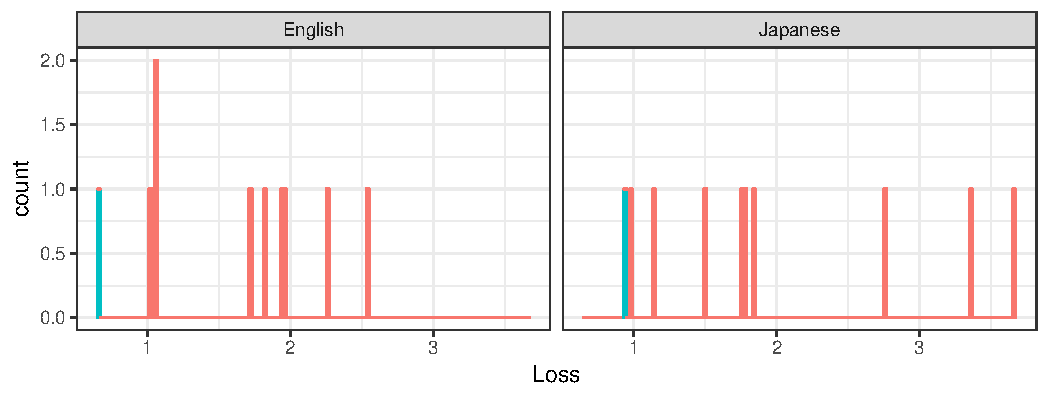
\includegraphics[scale=.7]{figures/cky-parse.pdf} 
	\caption{Parsability loss $H[T|L_\theta(T)]$ (lower is better) computed by a simple CKY parser, for random word order grammars (red) and word order grammars optimized for efficiency (blue).}
    \label{fig:cky-parser}
\end{figure}



\subsection{Distorted graph-based parsers}

Many of the word order biases explained by parseability in Table~\ref{tab:result-dryer} are also explained by dependency length minimization. Therefore, we address here the idea that the graph-based parser might have a built-in bias toward parses involving short dependencies, which we call a \key{locality bias}.

A simple way to eliminate or alter a locality bias for any parser would be to change the order in which the parser sees words. Suppose that a parser $P$ has a bias toward positing a dependency between a word and the immediate previous word. 

\paragraph{Even--odd order.} A sequence of $n$ words originally ordered as $w_1 w_2 w_3 w_4 \cdots w_n$ is reordered by separating the even and odd indices: $w_2 w_4 w_6 \cdots w_{n-1} w_1 w_3 w_5 \cdots w_n$ (assuming $n$ odd). Therefore all words that are adjacent in the original order will be separated by a distance of $\approx n/2$ in the distorted order, while all words of distance 2 in the original order will become adjacent.

\paragraph{Interleaving order.} In interleaving ordering, a sequence originally ordered as $w_1 w_2 w_3 \cdots w_n$ is split in half at the middle (index $m=\ceiling{n/2}$), and the two resulting sequences are interleaved, yielding $w_1 w_m w_2 w_{m+1} w_3 w_{m+3} \cdots w_n$. Thus all words that were originally adjacent will have distance 2 in the distorted order, with the intervening word coming from a very distant part of the sentence.

\paragraph{Inwards order.} A sequence originally ordered as $w_1 w_2 w_3 \cdots w_{n-1} w_n$ is ordered from the edges of the string inwards, as $w_1 w_n w_2 w_{n-1} \cdots w_{\ceiling{n/2}}$. This corresponds to folding the string in on itself once, or equivalently, splitting the sequence in half at the middle, then interleaving the two resulting sequences after reversing the second one. The result is that the most non-local possible dependencies in the original order become the most local dependencies in the distorted order.

\paragraph{Sorted order.} A sequence is reordered by sorting by POS tags, and randomizing the order within each block of identical POS tags.
To each word, we then add a symbol encoding the original position in the sequence.
For instance
\begin{center}
PRON VERB PRON
\end{center}
may be reordered as
\begin{center}
PRON 1 PRON 3 VERB 2
\end{center}
or
\begin{center}
PRON 3 PRON 1 VERB 2
\end{center}
The numbers are provided to the parser as atomic symbols from a vocabulary ranging from 1 to 200; numbers greater than 200 (which may occur in extremely long sentences) are replaced by an out-of-range token.


\paragraph{Experiments}
Using English and Japanese data, we trained parsers for the ten random word order grammars and for the best grammar optimized for efficiency, with the input presented in each of the distorted orderings.
Resulting parsing accuracy scores are shown in Figure~\ref{fig:distorted-parser}.
In all settings, the language optimized for efficiency achieved higher parsing accuracy than random ordering grammars, showing that the parser's preference for optimized languages cannot be attributed to a locality bias.
%Note that absolute values of parsing accuracy vary between the orderings, being higher for the actual orderings than for distorted orderings, in which trees become nonprojective.

\begin{figure}
    \centering
    English
    
    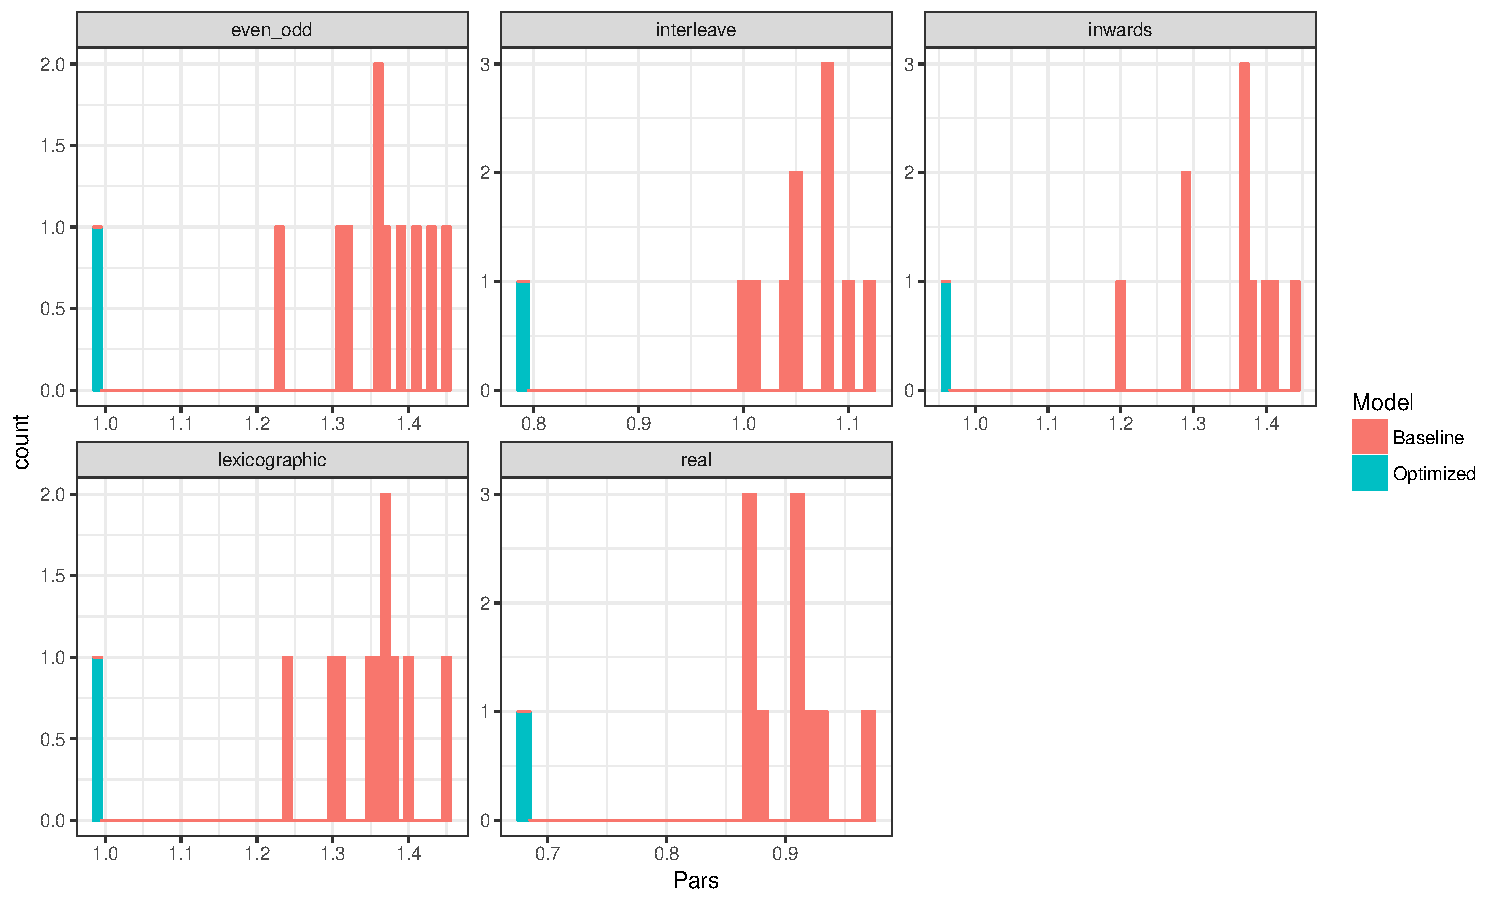
\includegraphics[scale=.5]{figures/adversarial-parse-loss-english.pdf}
    
    Japanese
    
    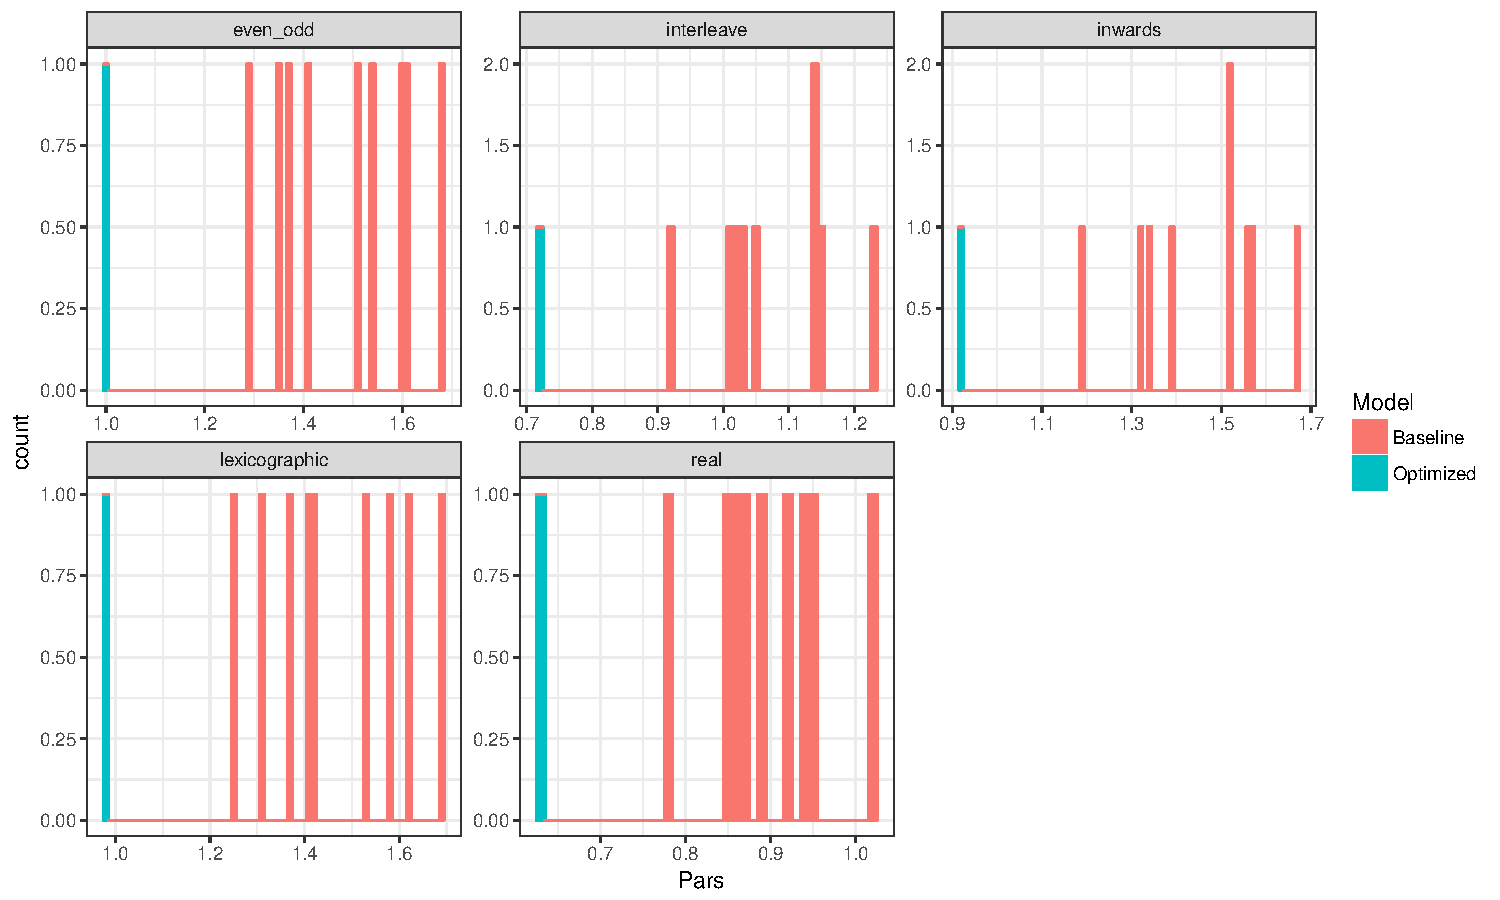
\includegraphics[scale=.5]{figures/adversarial-parse-loss-japanese.pdf}
	\caption{Parseability of baseline grammars and grammars optimized for efficiency, in English (top) and Japanese (bottom), measured by parsing loss $H[T|L_\theta(T)]$ (lower is better), for the four distorted orderings, and the actual orderings (`real').}
    \label{fig:distorted-parser}
\end{figure}


\subsection{n-gram language models}


We constructed a Bigram model with Kneser-Ney smoothing.
A bigram model predicts each word taking only the previous word into account.
This contrasts with LSTMs, which take the entire context into consideration.
Thus, bigram models and LSTMs stand on opposing ends of a spectrum of language models taking more and more aspects of the context into account.

We estimated language models on the training partitions, and used the validation partitions to estimate surprisal.
We conducted this for the ten random and the best optimized ordering grammars on English and Japanese data.
Results (Figure~\ref{fig:bigrams}) show that languages optimized for efficiency are optimal for a bigram language model.

\begin{figure}
    \centering
    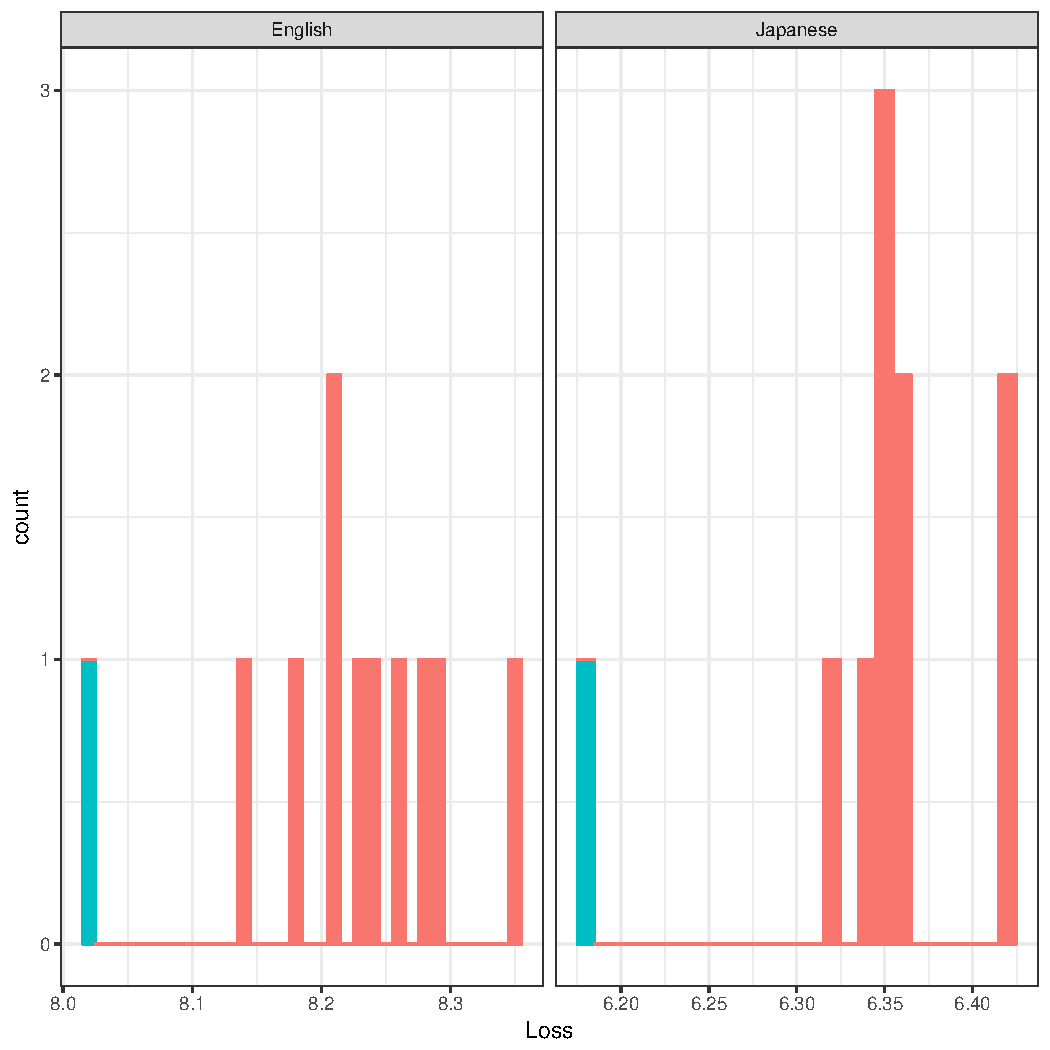
\includegraphics[scale=.4]{figures/bigrams.pdf} 
	\caption{Surprisal (lower is better) computed from Bigram model, on English and Japanese data ordered according to random ordering grammars (red) and ordering grammars optimized for efficiency (blue).}
    \label{fig:bigrams}
\end{figure}




\subsection{Discussion}

It is always a logical possibility in studies such as this one that the results are dependent on the particular probabilistic models used. 

\section{Effects of data sparsity}

Our efficiency objective comes down to 


If the difference between random and optimized languages is due to data sparsity, we expect that it decreases as the amount of training data is increased.
If, on the other hand, there is an inherent difference in efficiency between random and optimized languages, we expect that the difference persists as training data is increased.

We considered Czech, the UD language with the largest amount of available treebank data (approx. 2.2 Million words), up to $\approx$ 300 times more data than is available for some other UD languages.
We cosidered both a random ordering grammar, and the best ordering grammar optimized for parseabaility.
For both of these ordering grammars, we trained the parser on successively larger portions of the training data (0.1 \%, 1 \%, 5\%, 10\%, 20 \%, ..., 90 \%, 100 \%) and recorded parsing accuracy.
Furthermore, for the random grammar, we varied the number of neurons in the BiLSTM (200, 400, 800) to test whether results depend on the capacity of the network.


The resulting curves are shown in Figure~\ref{fig:learning-czech}.
A gap in parsing accuracy of about 0.07-0.1 appears already at 0.01 \% of the training data (2000 words), and persists for larger amounts of training data.

\begin{figure}
    \centering
    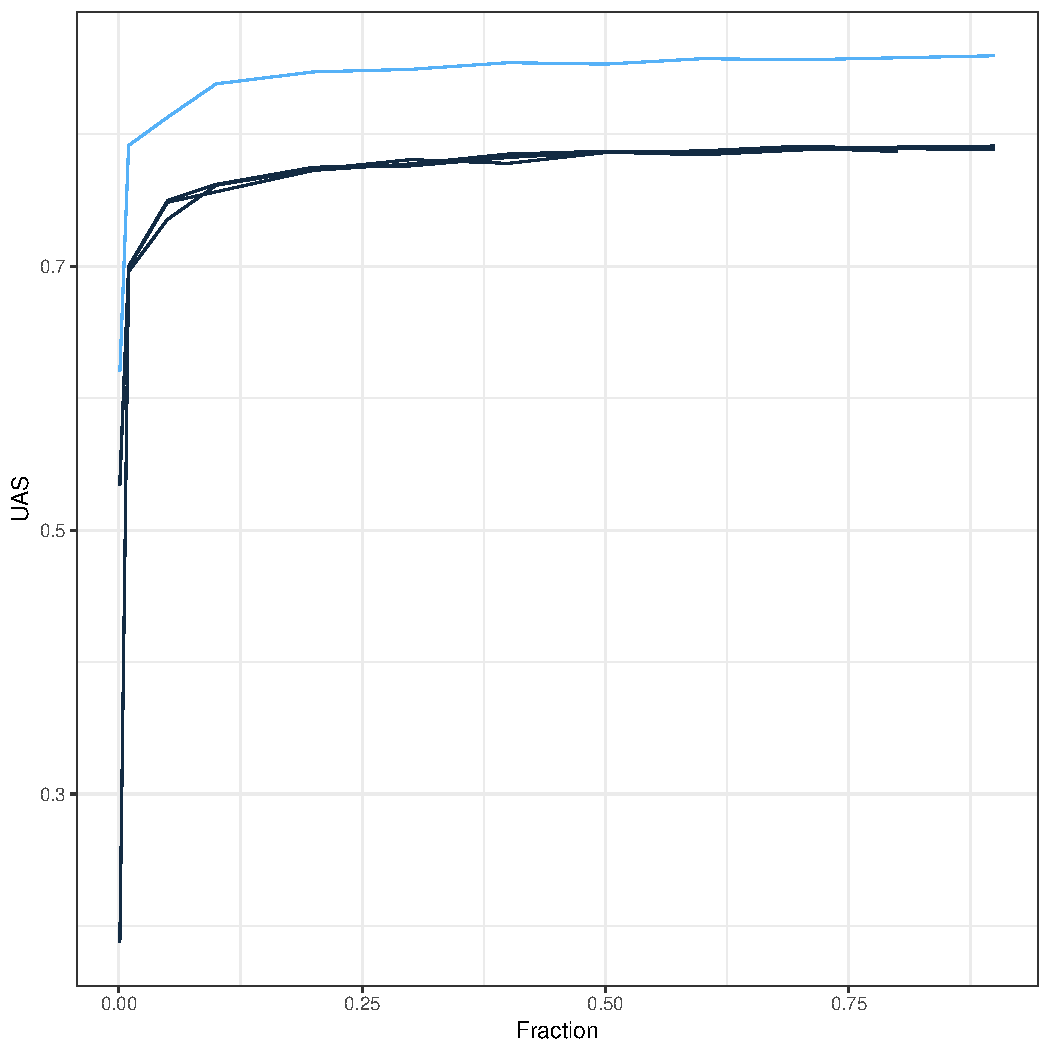
\includegraphics[scale=.4]{figures/learning-parser-czech.pdf} 
        \caption{Parsing accuracy (measured in UAS) for optimized (light blue) and random (black) ordering grammar on Czech data, as a function of the fraction of total training data provided.}
    \label{fig:learning-czech}
\end{figure}





\section{}




\bibliographystyle{acl_natbib}
\bibliography{everything}


\end{document}
